%%%%%%%%%%%%%%%%%%%%%%%%%%%%%%%%%%%%%%%%%%%%%%%%%%%%%%%%%%%%%%%%%%%%%%%%%%%%%%%%
%%
%%   BornAgain User Manual
%%
%%   homepage:   http://www.bornagainproject.org
%%
%%   copyright:  Forschungszentrum Jülich GmbH 2015
%%
%%   license:    Creative Commons CC-BY-SA
%%
%%   authors:    Scientific Computing Group at MLZ Garching
%%               C. Durniak, M. Ganeva, G. Pospelov, W. Van Herck, J. Wuttke
%%
%%%%%%%%%%%%%%%%%%%%%%%%%%%%%%%%%%%%%%%%%%%%%%%%%%%%%%%%%%%%%%%%%%%%%%%%%%%%%%%%


\chapter{Multilayer systems}  \label{sec:Multilayers}

\index{Multilayer|(}%
\index{Layer structures|see {Multilayer}}

Wave propagation through thin layers requires
a special formalism that accounts for
refraction and reflection (\cref{Swave21}).
The so obtained distorted plane waves are the base
for the reformulation of Born's scattering theory
in the distorted wave Born approximation (\cref{SDWBA}).
% TODO RESTORE XREF We also discuss the limits of coherent superposition (\cref{Scoherlen}),

\index{GISAS|see{Grazing-incidence small angle scattering}}

%%%%%%%%%%%%%%%%%%%%%%%%%%%%%%%%%%%%%%%%%%%%%%%%%%%%%%%%%%%%%%%%%%%%%%%%%%%%%%%%
\section{DWBA for layered samples}\label{Swave21}
%%%%%%%%%%%%%%%%%%%%%%%%%%%%%%%%%%%%%%%%%%%%%%%%%%%%%%%%%%%%%%%%%%%%%%%%%%%%%%%%

%--------------------------------------------------------------------------------
\begin{figure}[tb]
  \centering
    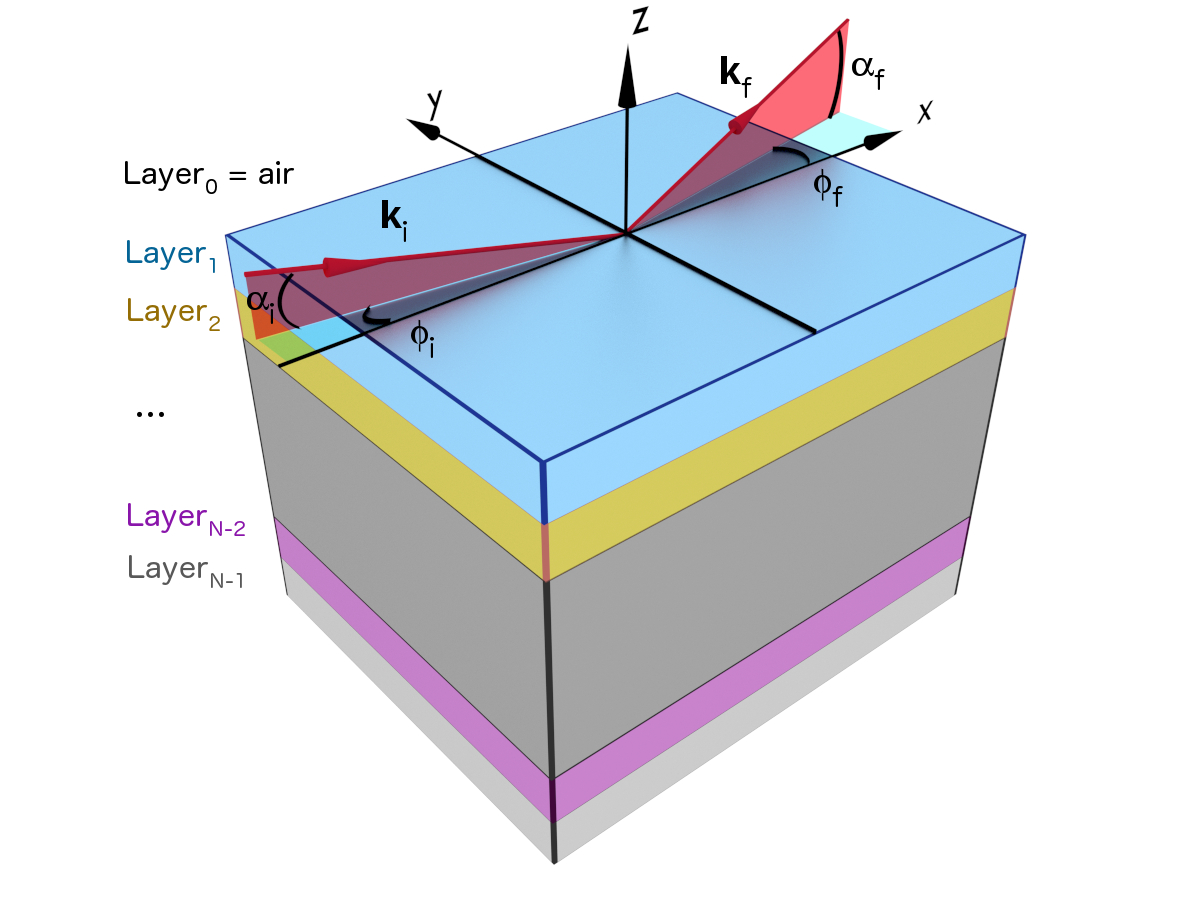
\includegraphics[clip=, width=120mm]{fig/drawing/setup_multilayer.jpg}
  \caption[Conventional GISAS scattering geometry.]{Geometric conventions
\index{Conventions!GISAS geometry}%
\index{Grazing-incidence small angle scattering!geometric conventions}%
\index{Coordinate system!GISAS geometry}%
\index{Glancing angle}%
\index{Scattering angles}%
\index{Geometry!conventions for GISAS}
  in GISAS scattering comprise a Cartesian coordinate system
  and a set of angles.
  The coordinate system has a $z$ axis normal to the sample plane,
  and pointing into the halfspace where the beam comes from.
  The $x$ axis usually points along the incident beam,
  projected onto the sample plane.
  Incident and final plane waves are characterized
  by wavevectors $\k_\ti$, $\k_\tf$;
  the angle $\alpha_\ti$ is the incident glancing angle;
  $\phi_\ti$ is usually zero, unless used to describe a sample rotation;
  $\alpha_\tf$ is the exit angle with respect to the sample's surface;
  and $\phi_\tf$ is the scattering angle with respect to the scattering plane.
  In the above figure $\phi_\tf$ is negative by convention, while all other angles
  are positive.
\nomenclature[1α024 2i000]{$\alpha_\ti$}{Glancing angle of the incident beam}
\nomenclature[1α024 2f000]{$\alpha_\tf$}{Glancing angle of the detected beam}
\nomenclature[1φ024 2i000]{$\phi_\ti$}{Angle between the incident beam, projected into the sample plane, and the $x$ axis}%
\nomenclature[1φ024 2f000]{$\phi_\tf$}{Angle between the detected beam, projected into the sample plane, and the $x$ axis}%
\nomenclature[2x020]{$x$}{Horizontal coordinate, usually chosen along the incoming beam projection}%
\nomenclature[2y020]{$y$}{Horizontal oordinate, chosen normal to $z$ and $x$}%
  The numbered layers illustrate a multilayer system as dicussed in \cref{sec:Multilayers}.
\index{Layer!numbering}%
\index{Multilayer}
  }
  \label{fig:expgeom}
\end{figure}
%--------------------------------------------------------------------------------

Reflectometry and grazing-incidence scattering
are designed for the investigation of surfaces, interfaces, and thin layers,
or most generically:
samples with a $2+1$ dimensional structure.
By convention,
we choose the sample surface to lie in the $xy$~plane,
\index{Sample plane}%
and its normal point out of the sample in positive $z$~direction.
\index{Sample normal}%
\nomenclature[2x020]{$x$}{Horizontal coordinate, in the sample plane}%
\nomenclature[2y020]{$y$}{Horizontal coordinate, in the sample plane}%
\nomenclature[2z020]{$z$}{Vertical coordinate, along the sample normal}%
\index{Horizontal plane}%
\index{Vertical direction}%
\index{Conventions|see {Horizontal and Vertical}}%
In our visualizations, we will always represent the $xy$~plane as \E{horizontal},
and the $z$~axis as upward \E{vertical},
altough there are ``horizontal'' reflectometers
where the sample normal is horizontal in laboratory space.
\index{Reflectometer!vertical vs horizontal}%

Scattering from such systems will be studied in distorted-wave Born approximation.
To determine the cross section~\cref{Exsection},
we need to determine the incident and final wavefunctions
$\psi_\si$ and~$\psi_\sf$.
Vertical variations of the refractive index $n(z)$
\index{Refractive index!vertical variation}%
cause refraction and reflection.
\index{Glancing angle}%
\index{Refraction}%
\index{Reflection}%
For waves propagating at small glancing angles,
the reflectance can take any value between 0 and~1,
even though $1-n$ is only of the order $10^{-5}$ or smaller.
Such zeroth-order effects cannot be accounted for
by perturbative scattering theory.
Instead, we need to deal with refraction and reflection
from the onset, in the wave propagation equation.

Therefore we have to modify our derivation of
the scattering cross section~\cref{Exsection} at an early stage,
namely at the decomposition~\cref{Edecompose_v} of the SLD.
\index{SLD!vertical variation}%
We specialize~\cref{Edecompose_v} to
\begin{equation}\label{Edecompose_vz}
  v(\r) = \mv(z) + \delta v(\r),
\end{equation}
allowing only vertical variations of~$\mv$.
Equations~\cref{Edispersion} and \cref{EnRefrIndx} must be modified
to allow for a $z$~dependence of the refractive index~$n(z)$ and the wavenumber~$K(z)$.
\index{Wave propagation!in multilayer|(}
The homogeneous wave equation~\cref{EHomoK} takes the form
\begin{equation}\label{EWaveZ}
  \left\{\Nabla^2+K(z)^2\right\}\psi(\r) = 0.
\end{equation}
Below and above the sample,
$K(z)=\text{const}$:
in these regions, $\psi(\r)$~is a superposition of plane waves.
The exciting wavefunction is
\index{Exciting wave!DWBA}%
\index{Wave!exciting}%
\begin{equation}\label{Epsiminus}
  \psi_\se(\r) = \e^{i\k_\parallel\r_\parallel+ik_{\perp\se}z},
\end{equation}
\nomenclature[0$\parallel$]{$\parallel$}{Parallel to the $xy$ sample plane}%
\nomenclature[0$\perp$]{$\perp$}{Normal to the $xy$ sample plane}%
\nomenclature[2k021\perp]{$k_\perp$}{Component of $\k$ along the sample normal}%
\nomenclature[2k041\parallel]{$\k_\parallel$}{Projection of $\k$ onto the sample plane}%
The subscripts $\parallel$ and~$\perp$ refer to the sample $xy$ plane.
The wave vector components $\k_\parallel$ and $k_{\perp}$ must fulfill
\begin{equation}
  K(z)^2=\k_\parallel^2+k_{\perp}^2.
\end{equation}
\index{Wavenumber!vertical}%
\index{Vertical wavenumber}%
Continuity across the sample implies
\begin{equation}\label{Ekconst}
  \k_\parallel = \text{const}.
\end{equation}
\index{Wavevector!horizontal!constant}%
\index{Horizontal wavevector!constant}%
When the incident wave hits the sample,
it is wholly or partly reflected.
Therefore, the full the solution of~\cref{EWaveZ} in the half space
of the radiation source is
\begin{equation}\label{Eref1}
  \psi(\r) = \e^{i\k_\parallel\r_\parallel+ik_{\perp\se} z} +
      R\, \e^{i\k_\parallel\r_\parallel-ik_{\perp\se} z}
\end{equation}
with a complex reflection coefficient~$R$.
\index{Reflection coefficient}%
The reflected flux is given by the re\-flect\-an\-ce $|R|^2$.
\index{Reflectance}%
\index{Flux!reflected}%
In the opposite halfspace, the solution of~\cref{EWaveZ} is simply
\begin{equation}\label{Etra1}
  \psi(\r) = T\, \e^{i\k_\parallel\r_\parallel+ik_{\perp\se} z}
\end{equation}
with a complex transmission coefficient~$T$.
The transmitted flux is given by the transmittance $|T|^2$.
\index{Transmittance}%
\index{Flux!transmitted}%

Within the sample, the wave equation~\cref{EWaveZ}
is solved by the factorization ansatz
\begin{equation}\label{Ekpar}
\psi(\r) = \e^{i \k_\parallel\r_\parallel} \phi(z).
\end{equation}
\nomenclature[1φ020 0z020]{$\phi(z)$}{$z$-dependent factor of $\psi(\r)$}%
The vertical wavefunction~$\phi(z)$
is governed by the one-dimensional wave equation
\begin{equation}\label{Ewavez}
\left\{\partial_z^2 + K(z)^2 - k_\parallel^2 \right\} \phi(z) = 0.
\end{equation}
As solution of a differential equation of second degree,
$\phi(z)$~can be written as superposition
of a downward travelling wave $\phi^-(z)$
and an upward travelling wave $\phi^+(z)$.
Accordingly, the three-dimensional wavefunction can be written as
\begin{equation}
  \psi(\r) = \psi^-(\r)+\psi^+(\r).
\end{equation}
\nomenclature[1ψ041 0\pm 2r040]{$\psi^\pm(\r)$}{Upward ($+$) or downward ($-$) propagating component of $\psi(\r)$}%
\nomenclature[0\pm]{$\pm$}{Upward ($+$) or downward ($-$) propagating}%
All this holds not only for the incident wavefunction~$\psi_\si$,
but also for the wavefunction~$\psi_\sf$
that is tracked back from a detector pixel towards the sample.
\index{Backtracing}%
\index{Scattered wave!backtracing}%
\index{Detector!backtracing}%
Accordingly,
the distorted-wave Born approximation will result in a cross section~\cref{Edwba}
that involves two incident and two final partial wavefunctions:
\index{Wave propagation!in multilayer|)}
\begin{equation}\label{Edwba4}
  \bra \psi_\ti|\delta v|\psi_\tf\ket
  = \bra \psi^-_\ti|\delta v|\psi^-_\tf\ket
  + \bra \psi^-_\ti|\delta v|\psi^+_\tf\ket
  + \bra \psi^+_\ti|\delta v|\psi^-_\tf\ket
  + \bra \psi^+_\ti|\delta v|\psi^+_\tf\ket,
\end{equation}
or in an obvious shorthand notation
\Emph{%
\begin{equation}\label{Edwba}
  \bra \psi_\ti|\delta v|\psi_\tf\ket
  = \sum_{\pm_\ti} \sum_{\pm_\tf}
    \bra \psi^\pm_\ti|\delta v|\psi^\pm_\tf\ket.
\end{equation}%
\vspace*{-5pt}}
This equation contains the essence of
the DWBA for GISAS,
and is the base for all scattering models implemented in \BornAgain.
Since $\bra \psi_\ti|\delta v|\psi_\tf\ket$
appears as a squared modulus
in the differential cross section~\cref{Exsection},
the four terms of \cref{Edwba} can interfere with each other,
which adds to the complexity of GISAS patterns.

%--------------------------------------------------------------------------------
\begin{figure}[tb]
\begin{center}
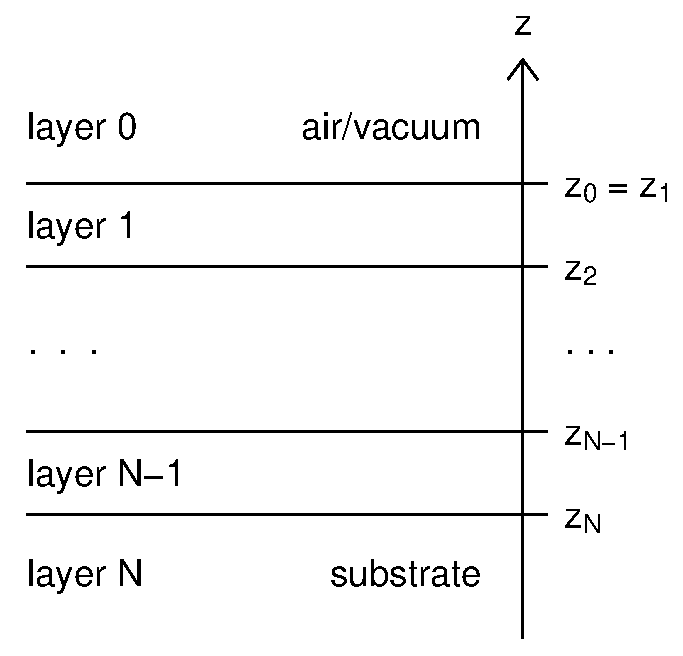
\includegraphics[width=0.4\textwidth]{fig/drawing/multilayer_z_conventions.ps}
\end{center}
\caption{Conventions for layer numbers and interface coordinates:
Layers are numbered from top to bottom.
The top vacuum (or air) layer (which extends to $z\to+\infty$) has number~0,
the substrate (extending to $z\to-\infty$) is layer~$N$.
\nomenclature[2n120]{$N$}{A multilayer sample has $N+1$ layers, including the
  semi-infinite bottom and top layers}
\index{Multilayer!numbering}%
\index{Layer!index}%
\index{Convention!layer number}%
The parameter $z_l$
\nomenclature[2z020 2l010]{$z_l$}{Vertical
  coordinate at the top of layer~$l$ (at the bottom for $l=0$)}%
is the $z$ coordinate of the \E{top} interface of layer~$l$,
\index{Multilayer!coordinates}%
\index{Layer!coordinate}%
\index{Convention!interface coordinate}%
except for $z_0$ which is the coordinate of the \E{bottom} interface
of the air or vacuum layer~0.}
\label{Fdefz}
\end{figure}
%--------------------------------------------------------------------------------


BornAgain supports multilayer samples
with refractive index discontinuities at layer interfaces.
Conventions for layer numbers and interface coordinates are
introduced in~\Cref{Fdefz}.
A multilayer sample consists of a finite sequence of discrete layers
$l=0,\ldots,N$
\nomenclature[2l010]{$l$}{Layer index}%
with constant refractive indices $n_l$
\nomenclature[2k122 2l010]{$K_l$}{Wavenumber in layer~$l$}%
\nomenclature[2n020 2l010]{$n_l$}{Refractive index of layer~$l$}%
and wavenumber $K_l\coloneqq K_\text{vac} n_l$.
Any up- or downward travelling solution of the wave equation shall be written
as a sum over partial wavefunctions,
\begin{equation}
  \psi^\pm(\r) = \sum_l \psi_l^\pm(\r),
\end{equation}
with the requirement
\begin{equation}
   \psi_l^\pm(\r) = 0 \text{~for $\r$ outside layer~$l$.}
\end{equation}
The DWBA matrix element~\cref{Edwba} then takes the form
\Emph{%
\begin{equation}\label{Edwbal}
  \bra \psi_\ti|\delta v|\psi_\tf\ket
  = \sum_l \sum_{\pm_\ti} \sum_{\pm_\tf}
    \bra \psi^\pm_{\ti l}|\delta v|\psi^\pm_{\tf l}\ket.
\end{equation}%
\vspace*{-5pt}}

%%%%%%%%%%%%%%%%%%%%%%%%%%%%%%%%%%%%%%%%%%%%%%%%%%%%%%%%%%%%%%%%%%%%%%%%%%%%%%%%
\section{Homogeneous layers}\label{SLayHomo}
%%%%%%%%%%%%%%%%%%%%%%%%%%%%%%%%%%%%%%%%%%%%%%%%%%%%%%%%%%%%%%%%%%%%%%%%%%%%%%%%

%===============================================================================
\subsection{DWBA for one layer}\label{SStep}
%===============================================================================

BornAgain currently only supports layers with a homogenous matrix.
In terms of~\cref{Edecompose_vz} this means that
$\mv(z)\eqqcolon v_l$ must be constant within a layer.

Within the layer, $\psi^\pm_l$ is a plane wave
that factorizes as in~\cref{Ekpar}.
Its amplitude~$A_l^\pm$ is determined recursively
by Fresnel's transmission and reflection coefficients
\index{Fresnel coefficients}%
that are based on continuity conditions at the layer interfaces.
This will be elaborated in \Cref{Sacrolay}.
\index{Multilayer!refractive index profiles}%
\index{Layer!refractive index profiles}%
The vertical wavenumber is determined by \cref{Epsiminus} and~\cref{Ekconst},
\begin{equation}
  k_{\perp l}^\pm = \pm\sqrt{K_l^2 - k_\parallel^2}.
\end{equation}
In the absence of absorption and above the critical angle,
wavevectors are real
so that we can describe the beam in terms of a glancing angle
\begin{equation}\label{Edef_alpha}
  \alpha_{\il}\coloneqq \arctan(k_{\perp \il}/k_{\plll}).
\end{equation}
Equivalently,
\begin{equation}
  k_{\plll}=K n_\il \cos\alpha_{\il}.
\end{equation}
Since $k_{\plll}$ is constant across layers,
we have
\begin{equation}\label{ESnell}
  n_\il \cos\alpha_{\il} = \text{the same for all }\il,
\end{equation}
which is Snell's refraction law.
\index{Refraction!Snell's law}
\index{Snell's law}
In general, however, the vertical wavenumber $k_{\perp}$,
determined by $K_l$ and $k_\parallel$ as per~\cref{Epsiminus},
can become imaginary (total reflection conditions) or complex (absorbing layer).
\index{Wavevector!complex}%
In these cases, glancing angles are no longer well defined,
and the geometric interpretation of~$\psi_l(\r)$ less obvious.
so that one has to fully rely on the algebraic formalism.

With the indicator function
\nomenclature[1χ032 2l010]{$\chi_l(z)$}{indicates whether $z$ is in layer~$l$}%
\index{Indicator function}%
\begin{equation}
  \chi_\il(\r)\coloneqq\left\{\begin{array}{ll}
  1&\text{~if $z_\il\le z \le z_{\il+1}$,}\\[.2ex]
  0&\text{~otherwise,} \end{array}\right.
\end{equation}
the vertical wavefunction can be written
\begin{equation}\label{Ephizwj}
  \phi^\pm_l(z)=A^\pm_l\e^{\pm ik_{\perp l}(z-z_\il)}\chi_l(z).
\end{equation}
\nomenclature[2a123 2w010 2l010 \pm]{$A^\pm_{w\il}$}{Amplitude
  of the plane wave $\phi^\pm_{w\il}(\r)$}%
The offset~$z_\il$ has been included in the phase factor for later convenience.

The DWBA transition matrix element~\cref{Edwba} is
\index{Distorted-wave Born approximation!multilayer}%
\begin{equation}\label{Edwba_ml0}
  \bra \psi_\ti|\delta v|\psi_\tf\ket
  = \sum_{\il} \sum_{\pm_\ti} \sum_{\pm_\tf}
    A^{\pm *}_{\ti \il} A^\pm_{\tf \il}
     \delta v_\il(\k^\pm_{\tf \il}-\k^\pm_{\ti \il})
\end{equation}
with the Fourier transform of the SLD
restricted to layer~$l$
\begin{equation}\label{Echij}
  \delta v_\il(\v{q})
  \coloneqq  \int_{z_\il}^{z_{\il-1}}\!\d z \int\!\d^2r_\plll\, \e^{i\v{q}\,\r}\delta v(\r)
  = \int\!\d^3r\, \e^{i\v{q}\,\r}\delta v(\r) \chi_l(z).
\end{equation}
\nomenclature[1δ00 2v030 2l010 2q040]{$\delta v_\il(\v{q})$}{Fourier transform
of the SLD $\delta v(\r)$, evaluated in one sample layer}%

To alleviate later calculations,
we now number the four DWBA terms from 1 to~4,
and define the corresponding wavenumbers and amplitude factors and as
\begin{equation}
  \begin{array}{l@{\hspace{2em}}l}
    \q^1 \coloneqq  \k^-_\tf - \k^-_\ti,& C^1 \coloneqq  A^{-*}_\ti A^-_\tf, \\[.6ex]
    \q^2 \coloneqq  \k^-_\tf - \k^+_\ti,& C^2 \coloneqq  A^{-*}_\ti A^+_\tf, \\[.6ex]
    \q^3 \coloneqq  \k^+_\tf - \k^-_\ti,& C^3 \coloneqq  A^{+*}_\ti A^-_\tf, \\[.6ex]
    \q^4 \coloneqq  \k^+_\tf - \k^+_\ti,& C^4 \coloneqq  A^{+*}_\ti A^+_\tf.
  \end{array}
\end{equation}
Accordingly, we can write \cref{Edwba_ml0} as
\Emph{
\begin{equation}\label{Edwba_ml}
  \bra \psi_\ti|\delta v|\psi_\tf\ket
  = \sum_{\il} \sum_{u} C^u_\il \delta v_\il(\q_\il^u).
\end{equation}
\vspace*{-5pt}}
Since $\k_\parallel=\text{const}$,
 all four wavevectors $\q^u$ have the same horizontal component;
they differ only in their vertical component~$q^u_\perp$.

%===============================================================================
\subsection{Wave amplitudes}\label{Sacrolay}
%===============================================================================

\index{Fresnel coefficients}%
\index{Transmission|see {Fresnel coefficients}}%
\index{Reflection|seealso {Fresnel coefficients}}%

The plane-wave amplitudes $A^\pm_{w\il}$ need to be computed recursively
from layer to layer.
Since these computations are identical for incident and final waves,
we omit the subscript~$w$ in the remainder of this section.
At layer interfaces, the optical potential changes discontinuously.
From elementary quantum mechanics we know that
piecewise solutions of the Schrödinger equations must be connected
such that the wavefunction $\phi(\r)$ and its first derivative
$\Nabla\phi(\r)$ evolve continuously.

% TODO REPLACE BY TEXT BELOW
\Note{Support for rough interfaces is already implemented in \BornAgain,
but documentation is adjourned to a later edition of this manual.}
%Unless layer interfaces are smooth,
%their roughness causes extra contribution to the total scattering.
%This is implemented in BornAgain as described in \Cref{SRough}.

To deal with the coordinate offsets introduced in \cref{Ephizwj},
we introduce the function%
\begin{equation}
  d_\il\coloneqq z_{\il}-z_{\il+1},
\end{equation}
which is the thickness of layer~$\il$,
except for $\il=0$,
where the special definition of $z_0$ (\cref{Fdefz}) implies $d_0=0$.
We consider the interface between layers $\il$ and $\il-1$,
with~$\il=1,\ldots,N$, as shown in \cref{Fboundary}.
This interface has the vertical coordinate $z_{\il}=z_{l-1}-d_{l-1}$.
Accordingly, the continuity conditions at the interface are
\begin{equation}\label{Econtcond}
  \begin{array}{lcl}
 \hphantom{\partial_z}\phi_{\il}(z_{\il}) &=& \hphantom{\partial_z}\phi_{\il-1}(z_{\il-1}-d_{\il-1}),\\
           \partial_z \phi_{\il}(z_{\il}) &=&           \partial_z \phi_{\il-1}(z_{\il-1}-d_{\il-1}).
  \end{array}
\end{equation}
We abbreviate
\begin{equation}
  f_\il \coloneqq  k_{\perp \il}/K = \sqrt{\nzj-(k_\plll/K)^2}
\end{equation}
and
\begin{equation}
   \delta_\il \coloneqq  \e^{iKf_\il d_\il}.
\end{equation}
For the plane waves \cref{Ephizwj},
the continuity conditions~\cref{Econtcond} take the form
\begin{equation}\label{Econt2}
  \begin{array}{@{}l@{}lcl@{}l}
  +A^-_{\il} &+A^+_{\il}
  &=&
  +A^-_{\il-1}\delta_{\il-1} &+A^+_{\il-1}\delta_{\il-1}^{-1},
  \\
  -A^-_{\il} f_{\il}  &+A^+_{\il} f_{\il}
  &=&
  -A^-_{\il-1}\delta_{\il-1} f_{\il-1} &+A^+_{\il-1}\delta_{\il-1}^{-1} f_{\il-1}.
  \end{array}
\end{equation}
After some lines of linear algebra,
we can rewrite this equation system as
\begin{equation}\label{EcMc}
  \left( \begin{array}{c}A^-_{\il-1}\\ A^+_{\il-1}\end{array} \right)
  = M_{\il} \left( \begin{array}{c}A^-_{\il}\\A^+_{\il}\end{array} \right)
\end{equation}
with the transfer matrix
\begin{equation}\label{EMil}
  M_\il
   \coloneqq
   \left(\begin{array}{cc}
     \delta_{\il-1}^{-1}&0\\
       0 & \delta_{\il-1}
   \end{array}\right)
   \frac{1}{2f_{\il-1}}
   \left(\begin{array}{cc}
       (f_{\il-1}+f_{\il})&(f_{\il-1}-f_{\il})\\
       (f_{\il-1}-f_{\il})&(f_{\il-1}+f_{\il})
   \end{array}\right).
\end{equation}

%--------------------------------------------------------------------------------
\begin{figure}[tb]
\begin{center}
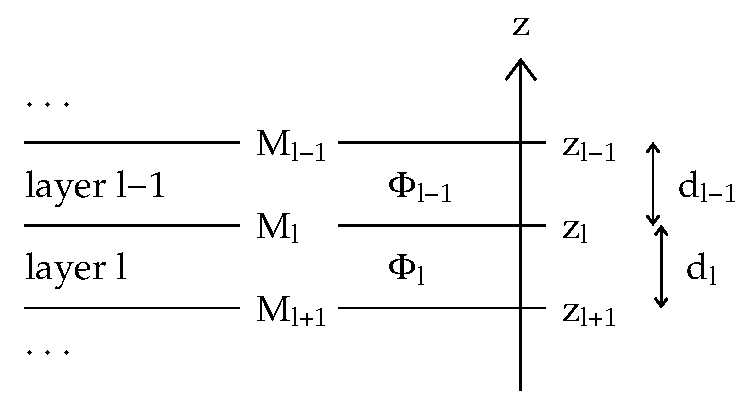
\includegraphics[width=0.46\textwidth]{fig/drawing/multilayer_boundary.ps}
\end{center}
\caption{The transfer matrix $M_l$ connects the wavefunctions
\index{Multilayer!transfer matrix}%
\index{Layer!transfer matrix}%
\index{Transfer matrix}%
$\Phi_l$, $\Phi_{l-1}$ in adjacent layers.}
\label{Fboundary}
\end{figure}
%--------------------------------------------------------------------------------

In a scattering setup,
plane-wave amplitudes are subject to two boundary conditions.
Let us assume that the source or the sink is located at $z>0$.
Then in the top layer, $A^-_{0}=1$ is given by the
incident or back-traced final plane wave.
In the substrate, $A^+_{N}=0$ because there is no radiation
coming from $z\to-\infty$.
This leaves us with two unkown amplitudes,
the overall coefficients of transmission~$A^-_N$ and reflection~$A^+_0$.
These two unknowns are  connected by a system of two linear equations,
\begin{equation}
  \left( \begin{array}{c}1\\ A^+_0\end{array} \right)
  = M_1 \cdots M_{N} \left( \begin{array}{c}A^-_N\\0\end{array} \right).
\end{equation}
While it is possible in principle
to solve this as a matrix equation,
the actual implementation in \BornAgain\
%\footnote{SpectralMatrix.cpp: SpectralMatrix::execute()}
starts with a unit vector in the substrate,
and then carries out the propagation step \cref{EcMc}
interface by interface,
yielding unnormalized amplitudes
\begin{equation}\label{EAtildel}
  \left( \begin{array}{c}\tilde A^-_{\il}\\ \tilde A^+_{\il}\end{array} \right)
  \coloneqq M_{\il+1}\cdots M_{N} \left( \begin{array}{c}1\\0\end{array} \right).
\end{equation}
When the top layer is reached,
the obtained values are normalized
so that the boundary condition $A^-_{0}=1$ be satisfied,
\begin{equation}
  A^\pm_{\il} = \frac{\tilde A^\pm_l}{\tilde A^-_0}.
\end{equation}
For GISAS detection in transmission geometry
\index{Transmission geometry}%
\index{Detector!transmission geometry}%
(sink location $z<0$) all the development
following \cref{EMil} holds with exchanged order of layers:
$(0,\ldots, N) \mapsto (N,\ldots,0)$.

\Work{GISAS in transmission geometry is not yet implemented in \BornAgain,
  but high on our agenda.}

At this point,
it may be an interesting exercise to make
 a connection with a well known textbook result.
Consider a system
with a single interface between two semi-infinite,
non-absorbing media. The incoming wave is assumed to be above the
critical angle, ensuring all $f_l$ are real.
The reflected flux,
normalized to the incident vertical flux $J_{0\perp}^-=-Kf_0$,
is
\index{Reflected flux}%
\begin{equation}
  \frac{J_{0\perp}^+}{J_{0\perp}^-}
  = - \left(\frac{f_0-f_1}{f_0+f_1}\right)^2,
\end{equation}
and the transmitted flux
\index{Transmitted flux}%
\begin{equation}
  \frac{J_{1\perp}^-}{J_{0\perp}^-}
  = \frac{4f_0 f_1}{(f_0+f_1)^2}.
\end{equation}
This satisfies particle number conservation, $J_{0\perp}^-+J_{0\perp}^+=J_{1\perp}^-$,
and agrees with Fresnel's result for $s$-polarized light.\footnote
{See any optics textbook, e.g.\ Born~\&~Wolf \cite[ch.~1.5.2]{BoWo99}
  or Hecht \cite[ch.~4.6.2]{Hec02}.}

The above algorithm fails if $f_{\il}\to0$
because $M_{\il+1}$ becomes singular.
The general solution of \cref{Ewavez} will be a linear function of $z$:
\begin{equation}
  \phi_{\il}(z) = A^0_{\il} + A^1_{\il}z.
\end{equation}
In \BornAgain, such a linear wavefunction amplitude can not be handled by the form factors,
which are only defined in terms of plane waves with complex wavevector components.
The following cases are treated seperately:
\begin{itemize}
  \item There is only one layer: this is a trivial case whithout any need to calculate wave coefficients.
    The solution in the single layer is just the incoming/outgoing plane wave.
  \item The top layer of a multilayer has $f_0=0$: the limit $f_0\to0$ is well-defined and the
    solution is given by $A^+_0 = -A^-_0$ and $A^{\pm}_{\il}=0$ for $\il>0$.
    % The boundary condition in the substrate imposes a linear relation between the two coefficients
    % of the linear wavefunction amplitude in the top layer. Since the first order term has to vanish, all amplitudes vanish.
  \item $f_{\il}=0$ for a layer with $\il>0$: In this case $f_{\il}$ will be given a very small imaginary value,
    representing a slight absorption. However, this should be inconsequential because the index of refraction
    of non-vacuum layer always contains an absorptive component.
\end{itemize}

%===============================================================================
\subsection{Flux, evanescent waves}\label{SSpecial}
%===============================================================================

We write
\begin{equation}\label{Edecompkperp}
  k_\perp \eqqcolon k_\perp' + i k_\perp''
\end{equation}
for the decomposition into a real and an imaginary part.
Accordingly, full wavevectors have the decomposition
\begin{equation}
  \k^\pm
  \eqqcolon {\k^\pm}' + i{\k^\pm}''
  = \k_\plll \pm (k_\perp' + i k_\perp'')\v{\hat z}.
\end{equation}
Per \cref{Endb1}, we have $\beta\ge0$ and $\delta<1$,
from which it follows that $k_\perp''$ always has the same sign as $k_\perp'$.

After these preparations,
we can compute the flux~\cref{EdefJ}:
\begin{equation}
  \begin{array}{@{}l@{\;}l}
  \v{J}(\r)
  =&   \left|A^-\right|^2 \e^{+2k_\perp'' (z-z_l)} {\k^-}'
    + \left|A^+\right|^2 \e^{-2k_\perp''(z-z_l)} {\k^+}'
\\[2ex]
  &+ \left[
      A^-{A^+}^* \e^{-2ik_\perp'(z-z_l)} {\left(\k_\plll-ik_\perp''\v{\hat z}\right)}
    + \text{c.c.}
    \right].
  \end{array}
\end{equation}
The first two terms describe the exponential intensity decrease
due to absorption, while
the oscillatory term in square brackets
is responsible for waveguide effects in layers with finite thickness.

The flux can also be written in terms of the one-dimensional wavefunctions $\phi^{\pm}(z)$:
\begin{equation}
  \begin{array}{@{}l@{\;}l}
  \v{J}(\r) =& \left|\phi^+(z)+\phi^-(z)\right|^2\cdot\k_\plll \\
  &+ \left[ \left|\phi^+(z)\right|^2 k_\perp' - \left|\phi^-(z)\right|^2 k_\perp' +
  2\Im(\phi^-(z){\phi^+}^*(z))k_\perp'' \right]\cdot \v{\hat z}.
  \end{array}
\end{equation}
The first term denotes the horizontal component
of the flux and can be seen to consist of the product
of the particle density at position $z$ and the wavector $\k_\plll$.
The $z$-component consists of the difference
between the up- and downward travelling wave components
and an extra term that encodes the interference between them.

In the special case of a purely imaginary~$k_{\perp \il}$,
the flux becomes:
\begin{equation}
  \v{J}(\r) = \left| \psi \right|^2 \k_\plll + 2 \Im (A^-{A^+}^*) k_\perp''\v{\hat z}.
\end{equation}
This flux consists of two clearly distinct parts: an \E{evanescent wave},
\index{Evanescent wave}%
travelling horizontally
 and a vertical component that is independent of the $z$ position.
The vertical component is a necessary
 degree of freedom to fulfill the boundary conditions at the layer's top and bottom interfaces.
In the case of a semi-infinite layer, the vertical component becomes zero and
 all incoming radiation at the top of the layer undergoes \E{total reflection}.
\index{Total reflection}%


%===============================================================================
\iffalse
\section{Graded refractive index}\label{Sgraded}
%===============================================================================

\Cref{Ewavez} has no practicable solution for arbitrary functions~$K(z)$.

Within one layer, the refractive index must either be constant,
or have an affine linear dependence $n(z)^2=a+bz$.
All other cases must be handled by dividing the sample into many layers
and approximating $n(z)^2$ by a step function.

\Work{Support for linear gradings with $n(z)^2=a+bz$ is not yet implemented.}
\index{Refractive index!graded}%
\index{Graded layer}%
\index{Layer!graded}%

For a graded refractive index~$n$
 that is a smooth function of~$z$,
the differential equation~\cref{Ewavez} is best solved
using the WKB method.\footnote
{Also called \E{semiclassical approximation} or
\E{phase integral method},
%originally developed
%by Liouville (1837), Green (1837), Lord Rayleigh (1912), and Jeffreys (1923),
named after Wentzel (1926), Kramers (1926), Brillouin (1926).
See any textbook on quantum mechanics.}
\index{WKB method}%
\index{Semiclassical approximation|see {WKB method}}%
\index{Phase integral method|see {WKB method}}%

\fi

\index{Multilayer|)}%
